\chapter{Introduction}
\section{Motivation}
    
  % //TODO add more papers to where cameras are placed as I read more papers

  Reinforcement and Imitation Learning are the two most popular ways for robots to learn new tasks. In such scenarios they are usually fitted with cameras that allows them to judge and perceive their environment. These cameras can be mounted in many configurations: Mounted on their wrists \cite{chi2024UMIinthewild,openXEmbodimentRoboticLearning2024}, over the shoulder \cite{wang2024observeactasynchronousactive}, or in some cases placed around the environment \cite{exploringActiveVision2024chuang} that the robot is interacting to allow the entire scene to be observed. And these are not necessarily mutually exclusive, one can combine one or more of the mounting systems \cite{exploringActiveVision2024chuang} all in efforts to ensure the robot, while collecting data and learning a task, has the most unobstructed and complete information in order to \emph{understand} its surroundings and the scene.

  On this visual information we can train control policies for robots using Neural Networks \cite{spyros1995nnStateOfTheArt, Schmidhuber2015nn} -of differing architectures- that are fit for the task we need our robot to do. However, these methods of mounting cameras comes with various disadvantages:
  
  \textbf{Static Cameras} Environment observing static cameras, such as over-the-shoulder (third-person) mounted cameras mean that the robot is confined to its environment and occlusions are still possible depending on the angles and the number of such cameras placed.
    
  \textbf{Camera-in-hand} This method can suffer from similar issues. As the gripper is oriented to execute a task, the viewpoints the camera sees will change. This dependency means that select tasks that are inherently occluding, once the gripper is engaged; for example, screwing in a lightbulb, inserting a key \ldots This means that optimal learning cannot be achieved for such a robot. As we get partial observability of the Region of Interest (ROI) at best and complete occlusion of the ROI at worst. See example in Figure \ref{fig:ex-occlusion} and Figure \ref{grid-occlusion}.

  \begin{figure}[h]
    \centering
    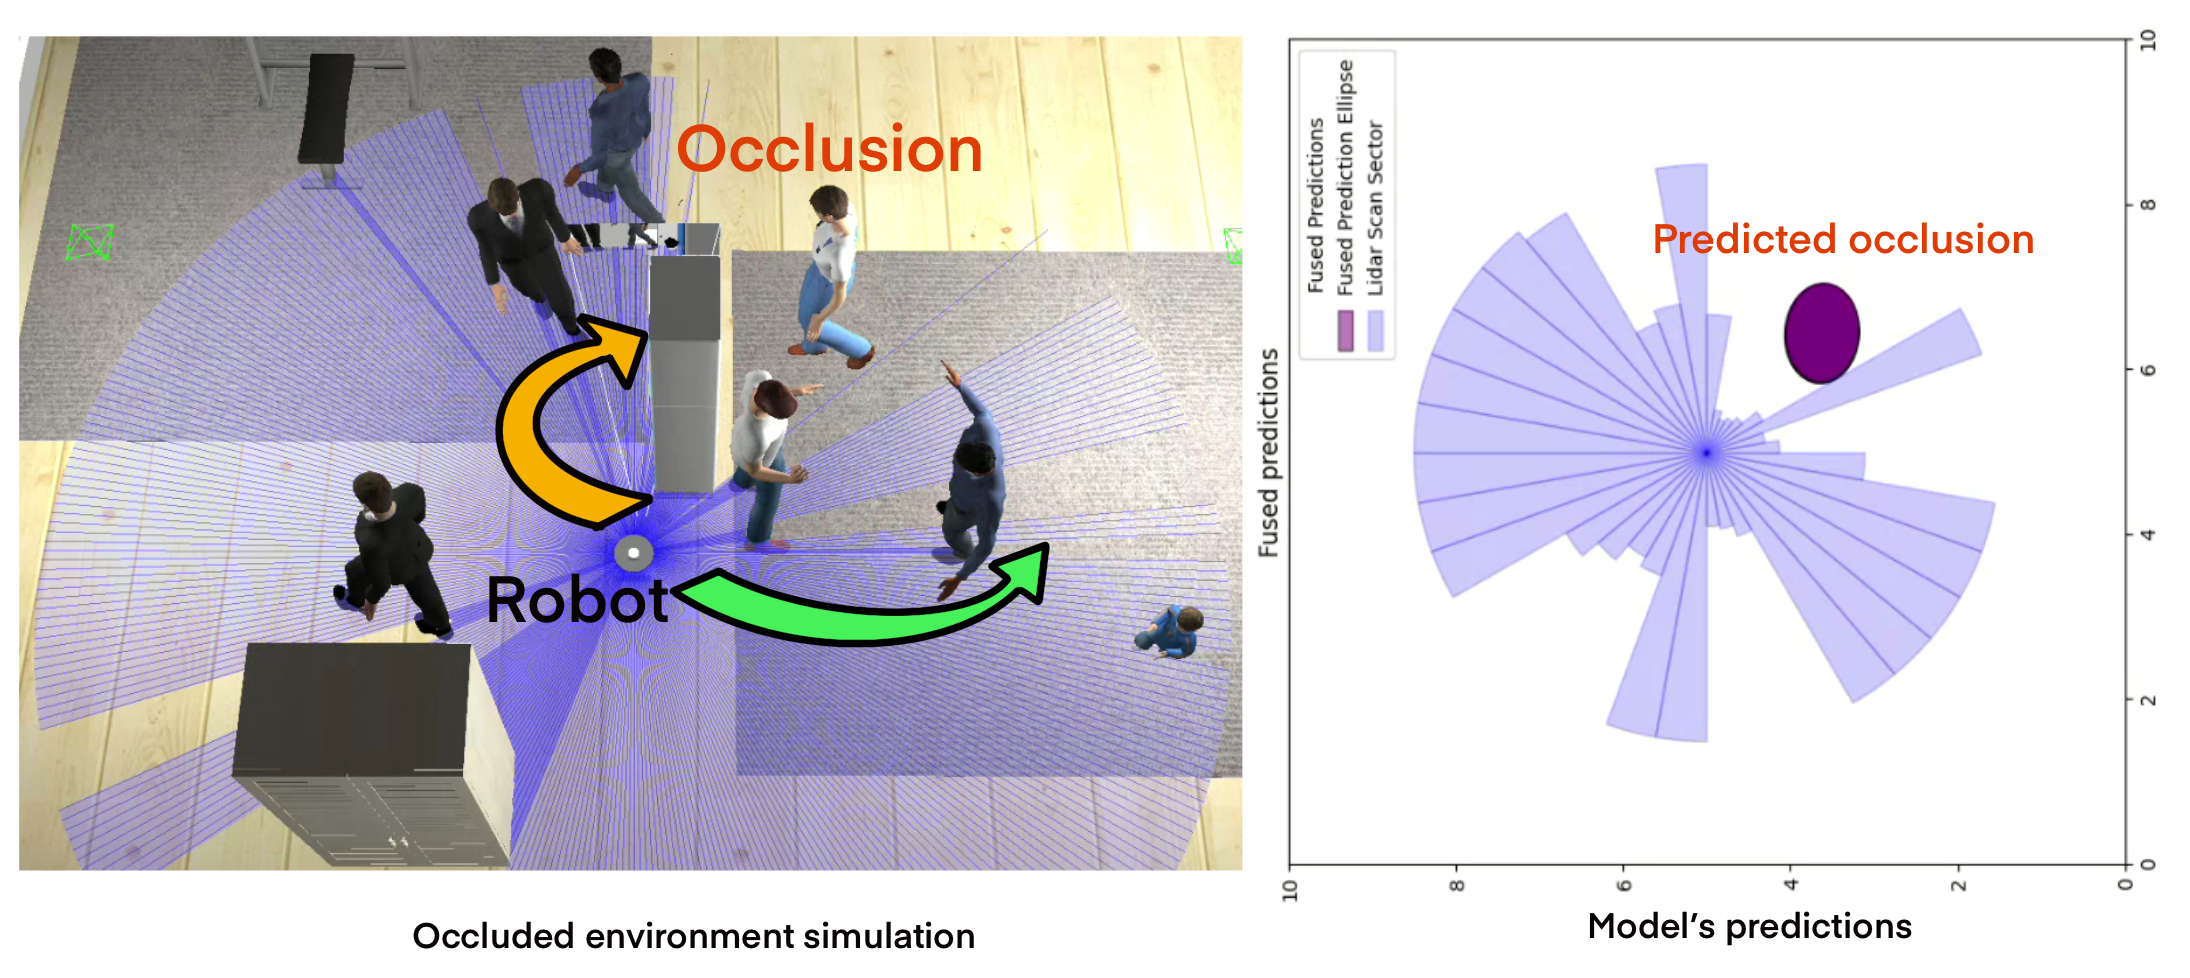
\includegraphics[width=0.7\textwidth]{assets/intro/intro-occlusion.png}
    \caption{Example of a robot mapping occluded areas \cite{ranaraja2024occlusionawareobstacleprediction}}\label{fig:ex-occlusion}
  \end{figure}
    
  In contrast to the above, us humans use our eyes which can be operated independently from our arms. This optimising aspect of human visual feedback \cite{findlay2003active,maiello2021humans,goodman2018using} is one of the cornerstones of human learning and environment manipulation. So, a possible remedy of the above issues is having a free moving, controllable camera alongside a interactive live (i.e. a gripper). This human-like setup -with the grippers as the arms and the camera arm as the neck, head and eyes- now allows our robot to find optimal camera poses for the tasks at hand and gain the most information about a scene.
  
  This now means that the \emph{visuomotor} tasks, where robot stimuli are controlled according to observations, shift to that of an \emph{Active Vision} one. This is a highly active area of research in robotics and mostly tackled through synchronous video with teleoperation \cite{exploringActiveVision2024chuang} with Behavioural Cloning, where a human \emph{pilot}will control the robot through some sort of interface, like a virtual reality (VR) headset. So the robot can learn to move its viewpoints according to this pilot's demonstrations. Another avenue of exploration is asynchronous vision, where the vision and movement information is learnt separately but coupled during execution of the robot \cite{natarajan2021graspsynthesisnovelobjects,wang2024observeactasynchronousactive}.


  \begin{figure}[h]
    \centering
    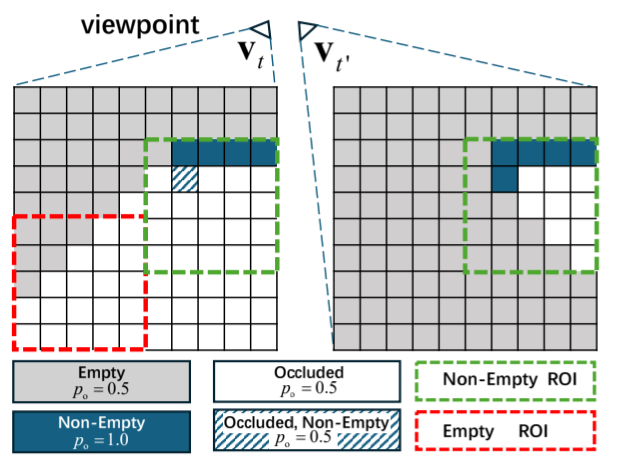
\includegraphics[width=0.8\textwidth]{assets/intro/grid-occluded.png}
    \caption{Example of multiple viewpoints gathering different information \cite{wang2024observeactasynchronousactive}}\label{fig:grid-occlusion}
  \end{figure}
  \todo[color=green]{make a better image for final}

  So our goal in this project is to explore how a robot can learn end-to-end control policies while also learning an active vision policy to optimise the movement of the camera during execution of tasks. And how this compares to existing methods of learning policies, with or without active vision approaches, and possibly its prevalence in real world scenarios. 

\section{Objectives}\label{sec:intro-objectives}
    So, the plan of this project then is to investigate whether a robot can be made to learn an active vision policy around the task it is currently being instructed (Imitation) or is currently exploring with some reward (Reinforcement).
    \todo[color=green]{Could change depending on where we get to exploring, I think the intereting ones are 2 and 3, 1 seems to be done a few times}

    We are therefore proposing three ways to investigate this:
    \begin{enumerate}
      \item Robot learns a policy as normal. Then during policy execution, the robot uses 3D-reasoning and forward planning, in order to predict its optimal pose so that the object(s) of interest are clearly visible and not occluded by other objects.
      \item The robot randomly moves its camera around during the policy learning in order to generate a range of different camera viewpoints (for the same robot states). When the policy is deployed, the uncertainty of the policy can be used to guide the camera towards regions with low uncertainty.
      \item In simulation, reinforcement learning is used to train a policy that directly controls the camera, for any given task and object, using randomly generated "pseudo-tasks". Then after training a robot on a task using human demonstrations in the real world. Two policies will be deployed: the main policy controlling the robot's hand, and the policy controlling the robot's camera.
\end{enumerate}
% \todo[color=green]{testing should be done on real life and simulated scenarios alike}
% Following on from the results of a predetermined test suite we can then determine what is the most promising model out of the three and develop them further.
% \section{Scope}
% \todo{Not sure if this is needed for Interim report, will come back}
% !!Not sure if this is needed, following are some things I thought could be included here for the final project report.

% \begin{itemize}
% 	\item Types of tasks the project will cover
% 	\item assumptions, camera, robot, arm types etc
% 	\item predetermined test suite maybe?
% 	\item distinction between control policies for the hand arm (policy for task) and the camera (optimal view)
% \end{itemize}

% \todo[color=red]{info edward wanted check teams}